\documentclass[12pt]{article}

\usepackage{graphicx}
\usepackage{enumitem}
\usepackage{amsmath}
\usepackage{gvv-book}
\usepackage{gvv}

\title{\textbf{1.8.22: Equidistant Points Problem}}
\author{\textbf{ee25btech11005 - Aditya Mishra}}
\date{September 9, 2025}

\begin{document}

\maketitle

\section*{Question}

Find all points that are equidistant from the points 
\[
\vec{A} = \myvec{-5 \\ 4}, \vec{B} = \myvec{-1 \\ 6}.
\]

How many such points exist?

\subsection*{Solution}

Let the desired point be 
\[
\vec{O} = \myvec{x \\ y}.
\]

The equidistance condition is:
\[
\norm{\vec{O} - \vec{A}} = \norm{\vec{O} - \vec{B}}.
\]

Squaring both sides:
\[
\norm{\vec{O} - \vec{A}}^2 = \norm{\vec{O} - \vec{B}}^2.
\]

Using vector dot product,
\[
(\vec{O} - \vec{A})^\top (\vec{O} - \vec{A}) = (\vec{O} - \vec{B})^\top (\vec{O} - \vec{B}).
\]

Expanding,
\[
\vec{O}^\top \vec{O} - 2 \vec{A}^\top \vec{O} + \vec{A}^\top \vec{A} = \vec{O}^\top \vec{O} - 2 \vec{B}^\top \vec{O}+ \vec{B}^\top \vec{B}.
\]

Canceling terms,
\[
-2 \vec{A}^\top \vec{O} + \vec{A}^\top \vec{A} = -2 \vec{B}^\top \vec{O} + \vec{B}^\top \vec{B}.
\]

Rearranged,
\[
2 (\vec{B} - \vec{A})^\top \vec{O} = \vec{B}^\top \vec{B} - \vec{A}^\top \vec{A}.
\]

Substituting values,
\[
\myvec{4 & 2} \myvec{x \\ y} = \frac{37 - 41}{2} = -2.
\]

Simplified line equation:
\[
2x + y = -1.
\]

\textbf{Number of such points:} Infinitely many points lying on the above line.

\begin{figure}[h]
\centering
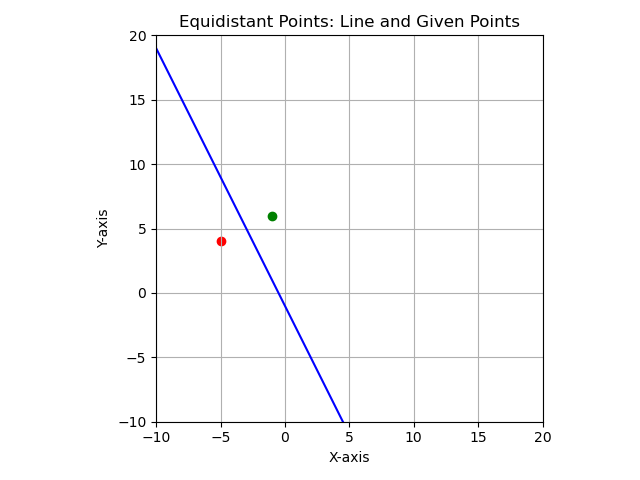
\includegraphics[width=0.8\columnwidth]{figs/equidistant_plot.png}
\caption{Points \(A, B\) and equidistant line \(2x + y = -1\).}
\label{fig:equidistant_plot}
\end{figure}

\end{document}
